\documentclass[10pt]{beamer}

\usepackage{lecture-style}

% title info
\title{Introduction to Computational Physics}

\author{\textbf{Jakub Rydzewski}\\[5pt]
  \footnotesize{\it NCU Institute of Physics}}

\date{\footnotesize\textcolor{gray}{Updated: \today}}

\begin{document}

% title page
{\setbeamertemplate{footline}{}\frame{\titlepage}}

\begin{frame}{Course Information}
\begin{itemize}
\setlength\itemsep{1em}
  \item Every Thursday at 14.15, online only
  \item GitHub link: \url{https://github.com/jakryd/0800-fizobl/}
  \item Slack group: \href{https://join.slack.com/t/ncu-students/shared_invite/zt-n1meknwx-_poiBXXMrYVbn9iHDj5rPw}{ncu-students/0800-fizobl-21}
  \item Zoom meeting ID: \href{https://zoom.us/j/2803172371?pwd=NVQ3c1FUZEZhNlZKaVZKSndHWjRaZz09}{208 317 2371}
  \item Exams take place in June 2021
\end{itemize}
\end{frame}

\begin{frame}{Outline}
\textcolor{subtitle}{Part 1. Statistical Mechanics}
\begin{itemize}
  \item Probability
  \item Phase space
  \item Thermodynamic equilibrium
  \item Statistical ensembles
\end{itemize}
\vspace{0.5cm}

\textcolor{subtitle}{Part 2. Monte Carlo Methods}
\begin{itemize}
  \item Sampling probability distributions
  \item Importance sampling
\end{itemize}
\vspace{0.5cm}

\textcolor{subtitle}{Part 3. Molecular Dynamics}
\begin{itemize}
  \item Verlet integrator
  \item Force and energy
\end{itemize}
\end{frame}

\begin{frame}{Outline}
\textcolor{subtitle}{Part 4. Enhanced Sampling}
\begin{itemize}
  \item Rare events
  \item Collective variables
  \item Free energy
\end{itemize}
\vspace{0.5cm}

\textcolor{subtitle}{Part 5. Nonequilibrium Statistical Physics}
\vspace{0.5cm}

\textcolor{subtitle}{Part 6. Machine Learning}
\begin{itemize}
  \item Connection between machine learning and statistical physics
  \item Unsupervised learning
\end{itemize}
\end{frame}

\begin{frame}{Literature}
\begin{itemize}
\setlength\itemsep{1em}
  \item M.~E. Tuckerman, \textit{Statistical Mechanics: Theory and Simulation}, Oxford University Press (2016).
  \item D. Chandler, \textit{Introduction to Modern Statistical Mechanics}, Oxford University Press (1987).
  \item R.~K. Patria, P.~D. Beale, \textit{Statistical Mechanics}, Elsevier (2011).
  \item M. Toda, R. Kubo, N. Saito, \textit{Statistical Physics I: Equilibrium Statistical Mechanics}, Springer-Verlag (1983).
  \item R. Kubo, M. Toda, N. Hashitsume, \textit{Statistical Physics II: Nonequilibrium Statistical Mechanics}, Springer-Verlag (1991).
\end{itemize}
\end{frame}

\begin{frame}{}
  \begin{center}
    \fontsize{25pt}{6}\selectfont\vspace{1.2cm}
    \textcolor{subtitle}{Statistical Mechanics}
  \end{center}
\end{frame}

\begin{frame}{Probability}
\begin{itemize}
\setlength\itemsep{1em}
  \item Probability is the language of statistical mechanics.
  \item Fundamental to the understanding of quantum mechanics.
  \item The large number of degrees of freedom of a macroscopic system make it necessary to use statistics.
\end{itemize}
\end{frame}

\begin{frame}{Probability}
\textbf{Random Variable}\vspace{0.2cm}
\emphbox{%
  A random variable $\boldsymbol{X}$ is completely defined by the range of values it can take, and its probability distribution $p_{\boldsymbol{X}}(x_1,\dots,x_k)$. The value $p_{\boldsymbol{X}}$ is the probability that the random variable $\boldsymbol{X}$ takes the value $\bx=(x_1,\dots,x_k)$.}
\vspace{0.2cm}

\begin{itemize}
\setlength\itemsep{1em}
  \item Note that $p_{\boldsymbol{X}}(\bx)\equiv\mathbb{P}[\boldsymbol{X}=\bx]$.

  \item From now on we write $p(\bx)$ to denote $p_{\mathbf{X}}(\bx)$.

  \item $p_{\boldsymbol{X}}(\bx)$ is non-negative and satisfies the normalization condition:
  \begin{equation}
    \int\d\bx\; p_{\boldsymbol{X}}(\bx)=1.
  \end{equation}

  \item The expectation value of $f(\boldsymbol{X})$ (or average) is denoted by:
  \begin{equation}
    \mathbb{E}[f]=\int\d\bx\; p_{\boldsymbol{X}}(\bx)f(\bx).
  \end{equation}
\end{itemize}
\end{frame}


\begin{frame}{Probability}
\textbf{Gaussian Random Variable $\boldsymbol{X} \sim \mathcal{N}(\boldsymbol{\mu}, \boldsymbol{\Sigma})$}\vspace{0.2cm}
\emphbox{A continuous variable $\boldsymbol{X}\in\mathbb{R}^k$ has a Gaussian distribution of mean $\boldsymbol{\mu}$ and variance $\boldsymbol{\sigma}^2$ if its probability density is:
\begin{equation}
  p(\bx) = \frac{\exp\left(-\frac{1}{2}(\bx-\boldsymbol{\mu})^{\mathrm{T}}\boldsymbol{\Sigma}^{-1}(\bx-\boldsymbol{\mu})\right)}{\sqrt{(2\pi)^k\det(\boldsymbol{\Sigma}})}.
\end{equation}
We have $\mathbb{E}[\boldsymbol{X}]=\boldsymbol{\mu}$ and $\textsf{Var}[\boldsymbol{X}]=\Sigma.$
}
\end{frame}

\begin{frame}{Probability}
\begin{itemize}
\setlength\itemsep{1em}
  \item The \textit{entropy} of a random variable $\boldsymbol{X}$ with probability distribution $p(\bx)$ is defined as:
  \begin{equation}
    H_{\boldsymbol{X}} \equiv - \int\d\bx\; p(\bx)\log p(\bx),
  \end{equation}
  where we define $0\log 0=0$.\fref{Units for $\log_2$: bits and $\log_\e$: nats}

  \item Entropy $H_{\boldsymbol{X}}$ is a measure of uncertainty of the random variable $\boldsymbol{X}$.
\end{itemize}
\end{frame}

\begin{frame}{Probability}
\textbf{Examples}\vspace{0.2cm}
\emphbox{%
  A fair coin has two values with equal probability. Its entropy is 1 bit.
}%
\vspace{0.2cm}
\emphbox{%
  Consider throwing $M$ fair coins: the number of all possible outcomes is $2^M$. The entropy equals $M$ bits.
}%
\vspace{0.2cm}
\emphbox{%
  \textit{Bernoulli process.} A Bernoulli random variable $X$ can take two values 0, 1 with probabilities $p(0)=q$ and $p(1)=1-q$. Its entropy is:
  \begin{equation}
    H_X = -q\log q - (1-q)\log(1-q).
  \end{equation}
  The entropy vanishes for $q=0$ or $q=1$ because the outcome is certain.
}
\end{frame}

\begin{frame}{Probability}
\begin{itemize}
\setlength\itemsep{1em}
  \item The Kullback-Leibler (KL) divergence (or the relative entropy) measures a stiatistical distance between $p(x)$ and $q(x)$. It is defined as:
  \begin{equation}
    D_{\mathrm{KL}}(q\|p) \equiv \int\d x\; q(x)\log\frac{q(x)}{p(x)}.
  \end{equation}

  \item $D_{\mathrm{KL}}(q\|p)$ is convex in $q(x)$,

  \item $D_{\mathrm{KL}}(q\|p) \geq 0$,

  \item and $D_{\mathrm{KL}}(q\|p)=0$ if $q(x)=p(x)$.

  \item Not symmteric: $D_{\mathrm{KL}}(q\|p) \neq D_{\mathrm{KL}}(p\|q)$.
\end{itemize}
\end{frame}

\begin{frame}{Dirac $\delta$ function}
\begin{itemize}
\setlength\itemsep{1em}
  \item $\delta(x)=0$ if $x \neq 0$ and $\delta(x) \rightarrow \infty$ (undefined) if $x=0$
  \item $\int_{-\epsilon}^{\epsilon}\d x\; \delta(x) = 1$ for all $\epsilon > 0$
  \item Gaussian model:
  \begin{equation}
    \delta_\sigma(x) = \lim_{\sigma \rightarrow 0} \frac{1}{\sqrt{2\pi\sigma^2}} \e^{-\frac{x^2}{2\sigma^2}}
  \end{equation}
\end{itemize}
\begin{figure}
  \includegraphics[width=0.4\textwidth]{fig/dirac-delta.png}
  \caption{Gaussian model for the Dirac $\delta$ function.}
\end{figure}
\end{frame}

\begin{frame}{Dirac $\delta$ function}
\begin{itemize}
\setlength\itemsep{1em}
  \item $\delta$ function times any arbitrary function $f(x)$ is:
  \begin{equation}
    \int_\infty^\infty \d x\; \delta(x)f(x) = f(0).
  \end{equation}

  \item Other models for $\delta$ function include Fourier integral:
  \begin{equation}
    \delta_\sigma(x) = \frac{1}{2\pi} \int_{-\infty}^\infty \d k\; \e^{ikx-|\sigma|x},
  \end{equation}
  and scaled sinc:
  \begin{equation}
    \delta_\sigma(x) = \frac{1}{\pi\sigma}\mathrm{sinc}(x/\sigma).
  \end{equation}

  \item Important for building histograms (notice the change of variables):
  \begin{equation}
    \int_{-\infty}^\infty \d x\; \delta(x-a)f(x) = f(a).
  \end{equation}
\end{itemize}
\end{frame}

\begin{frame}{Definitions}
\begin{itemize}
\setlength\itemsep{1em}
  \item \textit{Microscopic variable}: A variable pertaining to the individual atoms and molecules making up the system.

  \item \textit{Macroscopic variable}: A measurable quantity used to describe the state of the system. It depends collectively on the behavior of all the atoms and molecules. These arealso referred to as \textit{thermodynamic variables}.

  \item \textit{Extensive variables}: The system under consideration is often defined as encompassing some specific $N$ molecules. Then extensive variables are those whose magnitude is proportional to $N$.

  \item \textit{Intensive variables}: Those macroscopic variables whose magnitude is independent of $N$.
\end{itemize}
\end{frame}

\begin{frame}{Scales}
\begin{figure}
  \includegraphics[width=\textwidth]{fig/scales.jpg}
  \caption{Spatial and temporal scales.}
\end{figure}
\end{frame}

\begin{frame}{Phase Space}
\begin{figure}
  \includegraphics[width=0.5\textwidth]{fig/boltzman.png}
  \caption{Ludwig Boltzmann (1844--1906)}
\end{figure}
\end{frame}

\begin{frame}{Phase Space}
\begin{itemize}
\setlength\itemsep{1em}
  \item Consider a system with $N$ particles.
  \item Microscopic coordinates: $\br \equiv (r_1, \dots, r_{3N})$.
  \item Conjugate momenta: $\bp \equiv (p_1, \dots, p_{3N})$.
  \item We introduce the notion of generalized coordinates by stacking coordinates and momenta:
  \begin{equation}
    \bx \equiv (r_1, \dots, r_{3N}, p_1, \dots, p_{3N}).
  \end{equation}
  \item $\bx$ evolves in $\Gamma$ which defines the $6N$-dimensional \textit{phase space}.
\end{itemize}
\end{frame}

\begin{frame}{Phase Space}
\begin{figure}
  \includegraphics[width=0.7\textwidth]{fig/osc.png}
  \caption{Phase spaces of an undamped (blue) and a damped (orange) harmonic oscillator.}
\end{figure}
\end{frame}

\begin{frame}{Phase Space}
\begin{figure}
  \includegraphics[width=0.9\textwidth]{fig/osc-2.png}
  \caption{Phase spaces of the system.}
\end{figure}
\end{frame}

\begin{frame}{Ensemble Average}
\begin{itemize}
\setlength\itemsep{1em}
  \item \textit{Ergodicity hypothesis} -- the assumption that all states in an ensemble are reached by the time evolution of the corresponding system.
  \item We define the ensemble average of a quantity $A(\bx)$ as:
  \begin{equation}
    \left< A \right> = \frac{\int \d\bx\; A(\bx) \rho(\bx)}{\int \d\bx\; \rho(\bx)},
  \end{equation}
  where $\rho(\bx)$ is the phase space probability density.
\end{itemize}
\end{frame}

\begin{frame}{Hamiltonian}
\begin{itemize}
\setlength\itemsep{1em}
  \item The dynamics of the system under study is described by their \textit{Hamiltonian} $H(\bx)=\sum_{i=1}^N \frac{\bp_i^2}{2m_i} + U(\br)$.
  \item The equations of motion are:
  \begin{equation}
    \dot{p}_i = -\frac{\partial{H}}{\partial{r_i}}
    ~~~\mathrm{and}~~~
    \dot{r}_i = \frac{\partial{H}}{\partial{p_i}}~~~(i=1,\dots,3N).
  \end{equation}
  \item Can be rewritten as:
  \begin{equation}
    \dot{p}_i = -\frac{\partial{U}}{\partial{r_i}}
    ~~~\mathrm{and}~~~
    \dot{r}_i = \frac{p_i}{m_i},
  \end{equation}
  where $U(\br)$ is the potential energy.
\end{itemize}
\end{frame}

\begin{frame}{Liouville Theorem}
\begin{itemize}
\setlength\itemsep{1em}
  \item Temporal evolution of a phase space element of volume $V$ and boundary $\partial{V}$ is given by:
  \begin{equation}
  \label{eq:temp_ev}
    \frac{\partial}{\partial{t}} \int_V \d V\; \rho
      + \int_{\partial{V}}\d B\; \rho\bv = 0,
  \end{equation}
  where $\bv$ is a generalized velocity vector.

  \item In Eq.~\ref{eq:temp_ev}, $\rho$ satisfies the continuity equation:
  \begin{equation}
    \frac{\partial{\rho}}{\partial{t}} + \nabla\cdot(\rho\bv) = 0,
  \end{equation}
  which simplifies to ($\nabla\cdot\bv = 0$):
  \begin{equation}
    \frac{\partial{\rho}}{\partial{t}} = \{H, \rho\}
  \end{equation}
\end{itemize}
\end{frame}

\begin{frame}{Liouville Theorem}
\begin{itemize}
\setlength\itemsep{1em}
  \item The Liouville Theorem describes the time evolution of the phase space density $\dot{\rho} = \{H, \rho\}$.

  \item Poisson bracket: $\{u,v\} = \sum_i \left( \frac{\partial{u}}{\partial{r}_i}\frac{\partial{v}}{\partial{p}_i} - \frac{\partial{u}}{\partial{p}_i}\frac{\partial{v}}{\partial{r}_i} \right)$.
\end{itemize}
\begin{figure}
\centering
  \includegraphics[width=0.8\textwidth]{fig/vol-cons.png}
  \caption{Illustration of phase space volume conservation prescribed by Liouville's theorem.}
  \frefw{Source: M.~E. Tuckerman, \textit{Statistical Mechanics: Theory and Simulation}, Oxford University Press (2016).}
\end{figure}
\end{frame}

\begin{frame}{Thermodynamic Equilibrium}
\begin{itemize}
\setlength\itemsep{1em}
  \item In general, if $\rho(\bx, t)$ has an explicit time dependence, then so will an observable $A$.
  \item However, a system in thermodynamic equilibrium do not change in time, $\partial{\rho}/\partial{t}$ must be equal to 0.
  \item In such a case, no external forces act on the system.
  \item The Liouville equation reduces to:
  \begin{equation}
    \label{eq:eq-liouville}
    \{ \rho, H \} = 0.
  \end{equation}
\end{itemize}
\end{frame}

\begin{frame}{Thermodynamic Equilibrium}
\begin{itemize}
\setlength\itemsep{1em}
  \item The general solution to Eq.~\ref{eq:eq-liouville} is any function of $H$:
  \begin{equation}
    \label{eq:gen_sol}
    \rho(\bx) \propto F\left[H(\bx)\right].
  \end{equation}

  \item As $\rho$ needs to be properly normalized, we write the solutions as:
  \begin{equation}
    \rho(\bx) = \frac{1}{Z} F[H(\bx)],
  \end{equation}
  where $Z = \int\d\bx\; F[H(\bx)]$ is referred to as the \textit{partition function}.

  \item The partition function is a measure of the number of microscopic states in the phase space accessible within a given ensemble.

  \item Each ensemble has a particular partition function that depends on the macroscopic observables used to define the ensemble.
\end{itemize}
\end{frame}

\begin{frame}{Ensembles}
\begin{itemize}
\setlength\itemsep{1em}
  \item $N$ -- the number of particles, $V$ -- volume, $P$ -- pressure, $T$ -- temperature, $E$ -- internal energy.

  \item Microcanonical ensemble: constant $NVE$.

  \item Canonical ensemble: constant $NVT$.

  \item Canonical pressure ensemble: constant $NPT$.
\end{itemize}
\end{frame}

\begin{frame}{Microcanonical Ensemble}
\begin{itemize}
\setlength\itemsep{1em}
  \item $NVE$ are fixed, so also the probability density is constant:
  \begin{equation}
    \rho(\bx) = \frac{1}{Z} \delta[H(\bx) - E],
  \end{equation}
  where $\delta[\cdot]$ is the Dirac delta function and the microcanonical partition function is given by:
  \begin{equation}
    Z = \int \d\bx\; \delta[H(\bx) - E].
  \end{equation}

  \item We can see that the function $F[H(\bx)]$ from Eq.~\ref{eq:gen_sol} is:
  \begin{equation}
    F[H(\bx)] \propto \delta[H(\bx) - E].
  \end{equation}
\end{itemize}
\end{frame}

\begin{frame}{Microcanonical Ensemble}
\begin{itemize}
\setlength\itemsep{1em}
  \item State function is the entropy -- a quantity that can be related to the number of the microscopic states of the system.

  \item Control variables are:
  \begin{equation}
  \textstyle
    \frac{1}{T}=\left( \frac{\partial{S}}{\partial{E}} \right)_{N, V},
    \frac{P}{T}=\left( \frac{\partial{S}}{\partial{V}} \right)_{N, E},
    \frac{\mu}{T}=-\left( \frac{\partial{S}}{\partial{N}} \right)_{V, E}.
  \end{equation}

  \item Let $\Omega$ be the number of microscopic states; the relation of $S$ to $\Omega$ is:
  \begin{equation}
    S(N, V, E) = k_{\mathrm{B}} \log \Omega(N, V, E),
  \end{equation}
  where $k_{\mathrm{B}}$ is Boltzmann's constant:
  \begin{equation}
    k_{\mathrm{B}}=1.3806505(24)\times 10^{-23}~\mathrm{J/K}.
  \end{equation}
\end{itemize}
\end{frame}

\begin{frame}{Canonical Ensemble}
\begin{itemize}
\setlength\itemsep{1em}
  \item $NVT$ are fixed.
\end{itemize}
\begin{figure}
\centering
  \includegraphics[width=0.5\textwidth]{fig/canonical.png}
  \caption{In a canonical ensemble setup, the system we study (system 1) is coupled to a heat reservoir (system 2) that guarantees a constant temperature.}
  \frefw{Source: M.~E. Tuckerman, \textit{Statistical Mechanics: Theory and Simulation}, Oxford University Press (2016).}
\end{figure}
\end{frame}

\begin{frame}{Canonical Ensemble}
\begin{itemize}
\setlength\itemsep{1em}
  \item At a given temperature $T$, the probability for a system to be in a certain configuration $\bx$ with energy $E(\bx)$ is:
  \begin{equation}
  \label{eq:boltz}
    \rho(\bx) = \frac{1}{Z} \e^{-\beta E(\bx)},
  \end{equation}
  where $\beta = \frac{1}{\kT}$ is the \textit{inverse temperature}\fref{$\beta\approx 0.4$ kJ/mol at 300 K.}, and the canonical partition function is:
  \begin{equation}
    Z = \int\d\bx\; \e^{-\beta E(\bx)}.
  \end{equation}

  \item The ensemble average of a quantity $A$ is given by:
  \begin{equation}
    \left< A \right> = \frac{1}{Z} \int\d\bx\; A(\bx) \e^{-\beta E(\bx)}.
  \end{equation}
\end{itemize}
\end{frame}

\begin{frame}{Canonical Ensemble}
\begin{itemize}
\setlength\itemsep{1em}
  \item We can derive Eq.~\ref{eq:boltz} by using the maximum entropy princliple. We know that:
  \begin{equation}
    \int\d\bx\;\rho(\bx) E(\bx) = U,
  \end{equation}
  and that $\rho$ must be normalized.

  \item We introduce the augumented function $J$:
  \begin{align}
    J &\equiv -k_\mathrm{B}\int\d\bx\;\rho(\bx)\log\rho(\bx) \\ &+ \lambda_1 \left(\int\d\bx\;\rho(\bx)E(\bx) - U\right) \\ &+ \lambda_0 \left(\int\d\bx\;\rho(\bx) - 1\right),
  \end{align}
  where $\lambda_0$ and $\lambda_1$ are the Lagrange multipliers.
\end{itemize}
\end{frame}

\begin{frame}{Canonical Ensemble}
\begin{itemize}
\setlength\itemsep{1em}
  \item Taking the functional derivative w.r.t. to $\rho$ and setting it to zero, we have:
  \begin{equation}
    \frac{\delta J}{\delta \rho} = -k_\mathrm{B} \log\rho(\bx) - k_\mathrm{B} + \lambda_1 E + \lambda_0 = 0,
  \end{equation}

  \item which implies that the maximum entropy distribution is:
  \begin{equation}
    \rho(\bx) = \lambda_1 \e^{\frac{-k_\mathrm{B}+\lambda_0+\lambda_1 E(\bx) }{ k_\mathrm{B} }},
  \end{equation}
  which translates to:
  \begin{equation}
    \rho(\bx) = Z \e^{\frac{ -k_\mathrm{B}+\lambda_0 }{ k_\mathrm{B} }}
  \end{equation}
  where $Z$ is the canonical partition function:
  \begin{equation}
    Z=\int\d\bx\; \e^{\frac{\lambda_1}{k_\mathrm{B}} E}.
  \end{equation}
\end{itemize}
\end{frame}

\begin{frame}{Canonical Ensemble}
\begin{itemize}
\setlength\itemsep{1em}
  \item We get that the density must have a form:
  \begin{equation}
    \rho(\bx) = \frac{1}{Z}\e^{\frac{\lambda_1}{k_\mathrm{B}} E(\bx)}
  \end{equation}
  and the entropy is:
  \begin{equation}
    S(\bx) = -\lambda_1 U + k_\mathrm{B}\log Z.
  \end{equation}

  \item We differentiate $S$ w.r.t. $U$ and apply $\d U = T\d S - P\d V$:
  \begin{equation}
    \frac{\d S}{\d U} = -\lambda_1 \equiv \frac{1}{T}
  \end{equation}
  from which we get that:
  \begin{equation}
    \frac{\lambda_1}{k_\mathrm{B}} = -\frac{1}{k_\mathrm{B}T} = -\beta.
  \end{equation}
\end{itemize}
\end{frame}

\begin{frame}{}
  \begin{center}
    \fontsize{25pt}{6}\selectfont\vspace{1.2cm}
    \textcolor{subtitle}{Monte Carlo Methods}
  \end{center}
\end{frame}

\begin{frame}{Monte Carlo Methods}
The main steps of the Monte Carlo sampling are:
\vspace*{0.5cm}
\begin{itemize}
\setlength\itemsep{1em}
  \item Choose randomly a new configuration in phase space based on a Markov chain.
  \item Accept or reject the new configuration, depending on the strategy used.
  \item Compute the physical quantity and add it to the averaging procedure.
  \item Repeat the previous steps until convergence.
\end{itemize}
\end{frame}

\begin{frame}{Monte Carlo Methods}
\begin{equation}
  I = \int_0^1\d x \int_0^{\sqrt{1-x^2}}\d y = \frac{\pi}{4}
\end{equation}
\begin{figure}
\centering
  \includegraphics[width=0.99\textwidth]{fig/monte-carlo.png}
  \caption{Example of a Monte Carlo method to compute $\pi$.}
  \frefw{Source: \url{https://thatsmaths.com/2020/05/28/the-monte-carlo-method/}.}
\end{figure}
\end{frame}

\begin{frame}{Monte Carlo Methods}
\begin{itemize}
\setlength\itemsep{1em}
  \item The integrals that must be evaluated in equilibrium statistical mechanics are generally of the form:
  \begin{equation}
  \label{eq:general_int}
    I = \int\d \bx\; \phi(\bx) p(\bx),
  \end{equation}
  where $\bx$ is an $n$-dimensional vector, $\phi(\bx)$ is an arbitrary function, and $p(\bx)$ is a function satisfying the properties of a probability distribution:
  \begin{equation}
    p(\bx)\geq 0~~~\mathrm{and}~~~\int\d\bx\; p(\bx) = 1.
  \end{equation}

  \item Eq.~\ref{eq:general_int} represents the ensemble average of a physical observable in equilibrium statistial mechanics.
\end{itemize}
\end{frame}

\begin{frame}{Monte Carlo Methods}
\begin{itemize}
\setlength\itemsep{1em}
  \item Let $\bx_1, \bx_2, \dots, \bx_M$ be a set of $M$ $n$-dimensional vectors that are sampled from $p(\bx)$.

  \item The problem of sampling from $p(\bx)$ is a nontrivial one.

  \item For now, let us assume that such an algorithm exists. Then, an estimator:
  \begin{equation}
    \hat{I}_M = \frac{1}{M}\sum_{i=1}^M \phi(\bx_i)
  \end{equation}
  is such that:
  \begin{equation}
  \label{eq:est}
    \lim_{M\rightarrow\infty} \hat{I}_M = I.
  \end{equation}

  \item Eq.~\ref{eq:est} is guaranteed by the \textit{central limit theorem}.\fref{For the derivation, see M.~E. Tuckerman, \textit{Statistical Mechanics: Theory and Simulation}, Oxford University Press (2016), p.~281.}
\end{itemize}
\end{frame}

\begin{frame}{Monte Carlo Methods}
\begin{figure}
\centering
  \includegraphics[width=0.6\textwidth]{fig/clt-normal.png}
  \caption{Central limit theorem for a normal distribution.}
  \frefw{Source: \url{https://www.reddit.com/r/math/comments/2wrduu/central_limit_theorem/}.}
\end{figure}
\end{frame}

\begin{frame}{Monte Carlo Methods}
\begin{figure}
\centering
  \includegraphics[width=0.6\textwidth]{fig/clt-uniform.png}
  \caption{Central limit theorem for a uniform distribution.}
  \frefw{Source: \url{https://www.reddit.com/r/math/comments/2wrduu/central_limit_theorem/}.}
\end{figure}
\end{frame}

\begin{frame}{Monte Carlo Methods}
\begin{figure}
\centering
  \includegraphics[width=0.6\textwidth]{fig/clt-binom.png}
  \caption{Central limit theorem for a binomial distribution.}
  \frefw{Source: \url{https://www.reddit.com/r/math/comments/2wrduu/central_limit_theorem/}.}
\end{figure}
\end{frame}

\begin{frame}{Monte Carlo Methods}
\textbf{Central Limit Theorem}\vspace{0.2cm}
\emphbox{%
If $\bx_1, \bx_2, \dots, \bx_n$ are $n$ random variables drawn from a population with overall mean $\mu$ and finite variance $\sigma^2$, and if $\bar{\bx}_n$ is the sample mean, the limiting form of the distribution, $\lim_{n \rightarrow \infty} \sqrt{n} \left( \frac{\bar{\bx}_n - \mu}{\sigma} \right)$, is the standard normal distribution.}
\end{frame}

\begin{frame}{Monte Carlo Methods}
\begin{itemize}
\setlength\itemsep{1em}
  \item Example of sampling a simple distribution given by:
  \begin{equation}
    p(x) = c\e^{-cx},
  \end{equation}
  on the interval $x\in [0, \infty)$.

  \item To sample from $p(x)$, we need $P(X)$ such that:
  \begin{equation}
    \label{eq:cum}
    P(X) = \int_0^X \d x\; c\e^{-cx} = 1 - \e^{-cX},
  \end{equation}
  and equate Eq.~\ref{eq:cum} to a random number $\xi \in [0,1]$, then we can solve for X, which gives:
  \begin{equation}
    X = -\frac{1}{c}\log(1-\xi).
  \end{equation}

  \item In general, we do not have such simple distribution to sample from in statistical mechanics.
\end{itemize}
\end{frame}

\begin{frame}[fragile]{Monte Carlo Methods: Examples}
\begin{block}{Estimator no 1}
\begin{lstlisting}
def pi_estimator(n_samples):
  est = list()
  n_inside = 0; n_all = 0
  for i in range(n_samples):
    x = np.random.uniform(-1.0, 1.0)
    y = np.random.uniform(-1.0, 1.0)
    dist = np.sqrt(np.power(x, 2) +
                   np.power(y, 2))
    if dist <= 1.0:
      n_inside += 1
    n_all += 1
    est.append(4.0 * np.float(n_inside) /
               np.float(n_all))
  return np.array(est)
\end{lstlisting}
\end{block}
\end{frame}

\begin{frame}[fragile]{Monte Carlo Methods: Examples}
\begin{figure}
  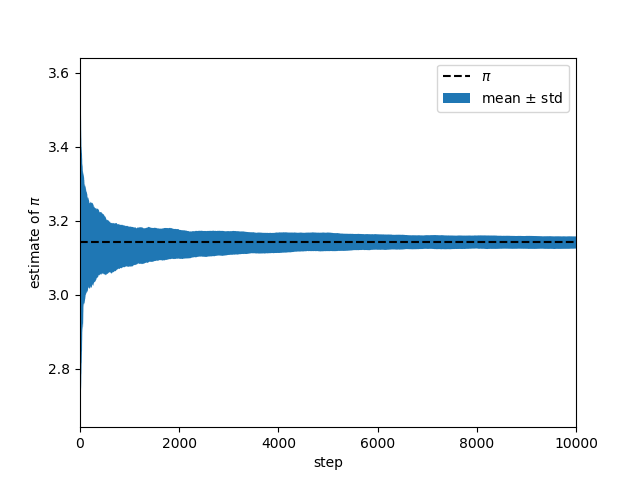
\includegraphics[width=0.8\textwidth]{code/fig/estimator-1.png}
  \caption{Estimator no 1.}
\end{figure}
\end{frame}

\begin{frame}[fragile]{Monte Carlo Methods: Examples}
\begin{block}{Estimator no 2}
\begin{lstlisting}
def pi_estimator_integral(n_samples):
  est = list()
  e = 0.0
  for i in range(n_samples):
    x = np.random.uniform(0.0, 1.0)
    y = 4.0 * np.sqrt(1.0 - np.power(x, 2))
    e += (y - e) / (np.float(i) + 1.0)
    est.append(e)
  return np.array(est)
\end{lstlisting}
\end{block}
\end{frame}

\begin{frame}[fragile]{Monte Carlo Methods: Examples}
\begin{figure}
  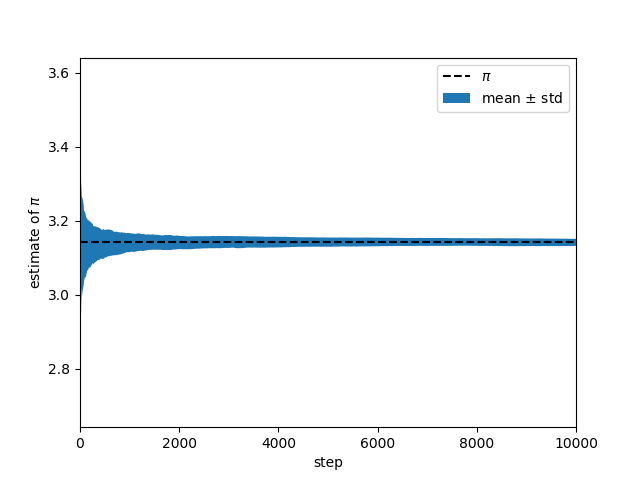
\includegraphics[width=0.8\textwidth]{code/fig/estimator-2.png}
  \caption{Estimator no 2.}
\end{figure}
\end{frame}

\begin{frame}[fragile]{Monte Carlo Methods: Examples}
\begin{block}{Estimator no 3}
\begin{lstlisting}
def pi_estimator_markov_chain(n_samples, step=0.1):
  est = list()
  n_inside = 0; n_all = 0;
  x = np.random.uniform(-1.0, 1.0)
  y = np.random.uniform(-1.0, 1.0)
  for i in range(n_samples):
    dx = np.random.uniform(-step, step)
    dy = np.random.uniform(-step, step)
    xn = x + dx; yn = y + dy
    if abs(xn) < 1.0 and abs(yn) < 1.0:
      x = xn; y = yn
    dist = np.sqrt(np.power(x, 2) + np.power(y, 2))
    if dist <= 1.0: n_inside += 1
    n_all += 1
    est.append(4.0 * np.float(n_inside) /
               np.float(n_all))
  return np.array(est)
\end{lstlisting}
\end{block}
\end{frame}

\begin{frame}[fragile]{Monte Carlo Methods: Examples}
\begin{figure}
  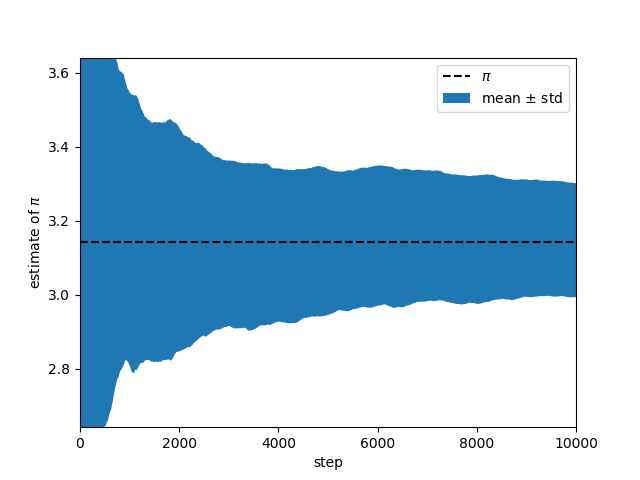
\includegraphics[width=0.8\textwidth]{code/fig/estimator-3.png}
  \caption{Estimator no 3.}
\end{figure}
\end{frame}

\begin{frame}{Importance Sampling}
\begin{itemize}
\setlength\itemsep{1em}
  \item However, instead of sampling $p(\bx)$ to estimate $\int\d\bx\; \phi(\bx) p(\bx)$, we could sample from a different distribution $b(\bx)$ by rewriting the integral as:
  \begin{empheq}[box=\boxeq]{equation}
    I = \int\d\bx\; \left[\frac{\phi(\bx) p(\bx)}{b(\bx)}\right] b(\bx).
  \end{empheq}

  \item We set $\psi(\bx) = \phi(\bx)p(\bx) / b(\bx)$ which gives us:
  \begin{align}
    I &= \int\d\bx\; \psi(\bx) b(\bx) \\ &\approx \frac{1}{M} \sum_{i=1}^M \psi(\bx_i),
  \end{align}
  where the vectors $\bx_i$ are sampled from $b(\bx)$.

  \item This trick is the basis of \textit{importance sampling}.
\end{itemize}
\end{frame}

\begin{frame}{Importance Sampling}
\begin{itemize}
\setlength\itemsep{1em}
  \item Using $b(\bx)$ as an importance function may lead to easier sampling.

  \item But how do we select $b(\bx)$?

  \item Is there an optimal choice of $b(\bx)$? The best one leads to the smallest possible variance:
  \begin{equation}
    \textsf{Var}[b(\bx)] = \int\d\bx\; \psi^2(\bx) b(\bx) - \left( \int\d\bx\; \psi(\bx) b(\bx) \right)^2
  \end{equation}
  that gives us:
  \begin{equation}
  \label{eq:var}
    \int\d\bx\; \frac{\phi^2(\bx) p^2(\bx)}{b^2(\bx)} b(\bx) - \left( \int\d\bx\; \phi(\bx) p(\bx) \right)^2
  \end{equation}

  \item Minimize $\textsf{Var}$ w.r.t. $b(\bx)$ subject to the constraint $\int\d\bx\; b(\bx)=1$
\end{itemize}
\end{frame}

\begin{frame}{Importance Sampling}
\begin{itemize}
\setlength\itemsep{1em}
  \item From Eq.~\ref{eq:var}, we have:
  \begin{equation}
    F[b(\bx)] = \textsf{Var}[b(\bx)] - \lambda \int\d\bx\; b(\bx),
  \end{equation}
  where $\lambda$ is a Lagrange multiplier.

  \item Computing the functional derivative $\delta F/\delta b(\bx)$, we obtain:
  \begin{equation}
    \frac{\phi^2(\bx) p^2(\bx)}{b^2(\bx)} + \lambda = 0
  \end{equation}
  or
  \begin{equation}
    b(\bx) = \frac{1}{\sqrt{-\lambda}} \phi(\bx) p(\bx).
  \end{equation}
\end{itemize}
\end{frame}

\begin{frame}{Importance Sampling}
\begin{itemize}
\setlength\itemsep{1em}
  \item Normalizing $b(\bx)$, we have:
  \begin{equation}
    \int\d\bx\; b(\bx) = \frac{1}{\sqrt{-\lambda}} \int\d\bx\; \phi(\bx) p(\bx) = 1.
  \end{equation}

  \item Thus, the optimal choice for $b(\bx)$ is:
  \begin{empheq}[box=\boxeq]{equation}
    b(\bx) = \frac{\phi(\bx) p(\bx)}{I}.
  \end{empheq}

  \item But if we knew the integral value $I$, we would not need to perform the calculation...
\end{itemize}
\end{frame}

\begin{frame}{Importance Sampling: Examples}
\begin{figure}
  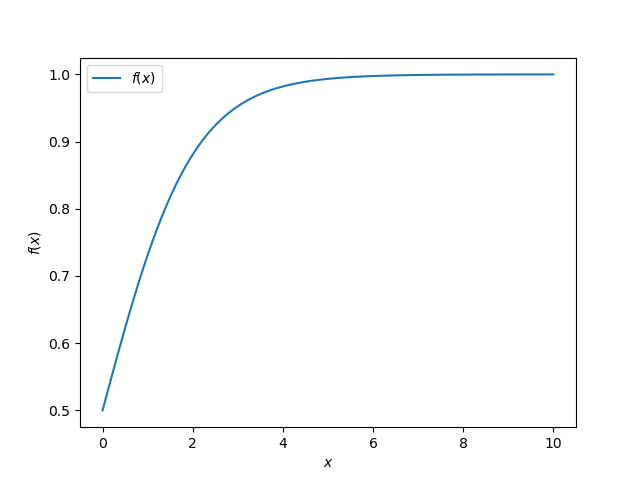
\includegraphics[width=0.8\textwidth]{code/fig/is_f.png}
  \caption{Function $f(x)=1/(1+\exp(-x))$.}
\end{figure}
\end{frame}

\begin{frame}{Importance Sampling: Examples}
\begin{figure}
  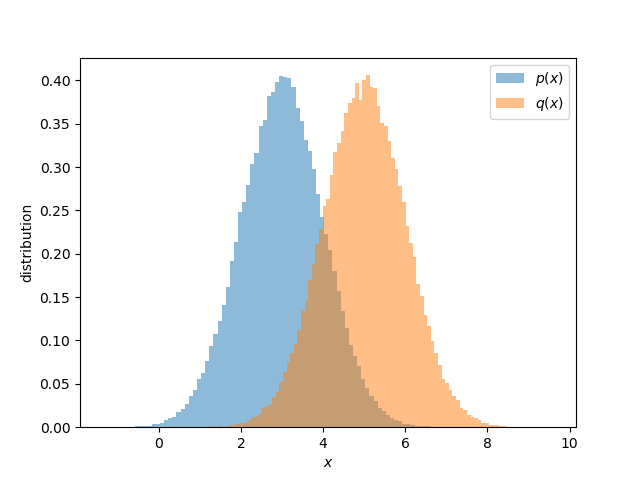
\includegraphics[width=0.8\textwidth]{code/fig/is_dist.png}
  \caption{Distributions to sample from.}
\end{figure}
\end{frame}

\begin{frame}{Importance Sampling: Examples}
\begin{figure}
  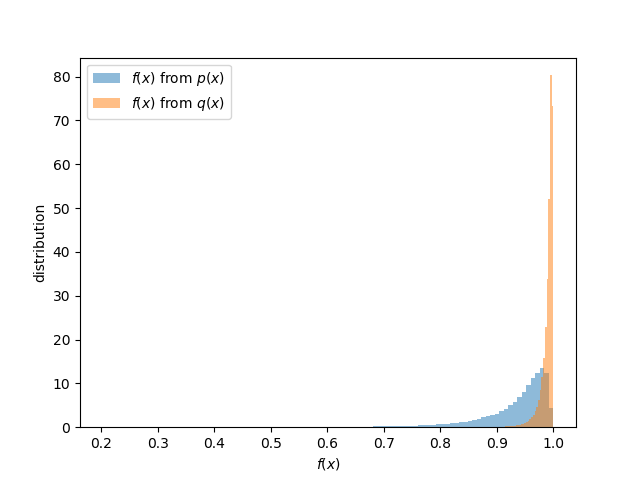
\includegraphics[width=0.8\textwidth]{code/fig/is_f_dist.png}
  \caption{Distributions of evaluated samples.}
\end{figure}
\end{frame}

\begin{frame}[fragile]{Importance Sampling: Examples}
\begin{block}{Results}
\begin{lstlisting}
python importance-sampling.py --n_samples 100000

f(x) from p(x): mean=0.9306712389 std=0.0686291035
f(x) from q(x): mean=0.9891990210 std=0.0132275039
f(x) from IS:   mean=0.9261305966 std=4.5258393804
\end{lstlisting}
\end{block}
\end{frame}

\begin{frame}{M(RT)$^2$}
\textbf{Markov Chain}\vspace{0.2cm}
\emphbox{
  If the vectors $\bx_1, \dots, \bx_M$ are generated sequentially, and $\bx_{i+1}$ is generated only based on the knowledge of $\bx_i$. the sequence is called a Makov chain.
}
\begin{figure}
  \includegraphics[width=0.7\textwidth]{fig/markov.jpg}
  \caption{Example of a simple Markov chain.}
\end{figure}
\end{frame}

\begin{frame}{M(RT)$^2$}
\begin{itemize}
\setlength\itemsep{1em}
  \item For physical systems, a Markov chain must satisfy the condition of \textit{detailed balance}, which ensures that the Markov process is microscopically reversible.

  \item M(RT)$^2$ is a rejection method.

  \item With the acceptance probability given by:
  \begin{equation}
    A(\bx_i | \bx_j) = \min\left[1, {f(\bx_i)}/{f(\bx_j)}\right],
  \end{equation}
  where $f(\bx)$ is the probability of the system being at $\bx$.

  \item Sampling in the canonical ensemble:\fref{Reminder: $\br$ are microscopic coordinates.}
  \begin{equation}
    A(\br_i | \br_j) = \min\left[1, \e^{-\beta \left[U(\br_i)-U(\br_j)\right]} \right],
  \end{equation}
  as $f(\br) \propto \e^{-\beta U(\br)}$.
\end{itemize}
\end{frame}

\begin{frame}[fragile]{Particle on Double-Well Potential}
\begin{lstlisting}
python mc-double-well.py --n_samples 10000 --temp 5
\end{lstlisting}
\vspace*{-0.3cm}
\begin{figure}
  \includegraphics[width=\textwidth]{code/fig/dw-pot.png}
\end{figure}
\end{frame}

\begin{frame}{Particle on Double-Well Potential}
\begin{figure}
  \includegraphics[width=\textwidth]{code/fig/dw-traj.png}
\end{figure}
\end{frame}

\begin{frame}{Particle on Double-Well Potential}
\begin{figure}
  \includegraphics[width=\textwidth]{code/fig/dw-hist.png}
\end{figure}
\end{frame}

\begin{frame}[fragile]{Particle on the M\"uller-Brown Potential}
\begin{lstlisting}
python mc-potential.py --n_samples 10000 --temp 1.0
\end{lstlisting}
\vspace*{-0.3cm}
\begin{figure}
  \includegraphics[width=\textwidth]{code/fig/mc-mb-t-1.png}
\end{figure}
\end{frame}

\begin{frame}[fragile]{Particle on the M\"uller-Brown Potential}
\begin{lstlisting}
python mc-potential.py --n_samples 10000 --temp 2.0
\end{lstlisting}
\vspace*{-0.3cm}
\begin{figure}
  \includegraphics[width=\textwidth]{code/fig/mc-mb-t-2.png}
\end{figure}
\end{frame}

\begin{frame}[fragile]{Particle on the M\"uller-Brown Potential}
\begin{lstlisting}
python mc-potential.py --n_samples 10000 --temp 3.0
\end{lstlisting}
\vspace*{-0.3cm}
\begin{figure}
  \includegraphics[width=\textwidth]{code/fig/mc-mb-t-3.png}
\end{figure}
\end{frame}

\begin{frame}[fragile]{Particle on the M\"uller-Brown Potential}
\begin{lstlisting}
python mc-potential.py --n_samples 10000 --temp 4.0
\end{lstlisting}
\vspace*{-0.3cm}
\begin{figure}
  \includegraphics[width=\textwidth]{code/fig/mc-mb-t-4.png}
\end{figure}
\end{frame}

\begin{frame}[fragile]{Particle on the M\"uller-Brown Potential}
\begin{lstlisting}
python mc-potential.py --n_samples 10000 --temp 5.0
\end{lstlisting}
\vspace*{-0.3cm}
\begin{figure}
  \includegraphics[width=\textwidth]{code/fig/mc-mb-t-5.png}
\end{figure}
\end{frame}

\begin{frame}{Replica Exchange Monte Carlo}
\begin{itemize}
\setlength\itemsep{1em}
  \item Barrier crossing are frequently rarely encountered during a simulation.

  \item For a barrier height of 15 kJ/mol at 300 K, the Boltzmann factor is approximately $3\times 10^{-3}$; for 30 kJ/mol is $6\times 10^{-6}$.
\end{itemize}
\begin{figure}
  \includegraphics[width=0.9\textwidth]{fig/barrier.png}
  \caption{Barrier crossing showing a trajectory in the case of a low and a high energy barrier, respectively.}
\end{figure}
\end{frame}

\begin{frame}{Parallel Tempering\fref{Marinari and Parisi. \textit{Simulated tempering: A new Monte Carlo scheme} Europhys. Lett. 19 (1992)}}
\begin{itemize}
\setlength\itemsep{1em}
  \item Temperature is used as the control variable, and different temperatures are assigned to the \textit{replicas}.

  \item In the parallel tempering scheme, a set of temperatures $T_1,\dots,T_M$ such that:
  \begin{equation}
    T_1 < T_2 < \dots < T_M
  \end{equation}
  are assigned to the $M$ replicas, where $T_1$ is the temperature $T$ of the canonical distribution.

  \item The high-temperature replicas easily cross potential energy barriers.

  \item We attempt exchanges between the neighboring replicas.
\end{itemize}
\end{frame}

\begin{frame}{Parallel Tempering}
\begin{figure}
  \includegraphics[width=\textwidth]{fig/pt-pes.png}
  \caption{Schematic of the parallel-tempering replica exchange Monte Carlo.\fref{Source: M.~E. Tuckerman, \textit{Statistical Mechanics: Theory and Simulation}, Oxford University Press (2016)}}
\end{figure}
\end{frame}

\begin{frame}{Parallel Tempering}
\begin{figure}
  \includegraphics[width=\textwidth]{fig/pt.png}
  \caption{An example of a parallel tempering trajectory.\fref{Source: \url{https://coulomb.umontpellier.fr/perso/daniele.coslovich/pt/}}}
\end{figure}
\end{frame}

\begin{frame}{Paralell Tempering}
\begin{itemize}
\setlength\itemsep{1em}
  \item Let $\br^{(1)}, \dots, \br^{(M)}$ be the complete configurations of the $M$ replicas, i.e., $\br^{(K)} \equiv (\br_1^{(K)}, \dots, \br_N^{(K)})$.

  \item The replicas are independent, so the total probability distribution $F(\br^{(1)}, \dots, \br^{(M)})$ is:
  \begin{equation}
    F(\br^{(1)}, \dots, \br^{(M)}) = \prod_{K=1}^{M} f_K\left( \br^{(K)} \right),
  \end{equation}
  where:
  \begin{equation}
    f_K\left( \br^{(K)} \right) = \frac{1}{Z} \e^{-\beta_K U\left( \br^{(K)} \right)},
  \end{equation}
  in which $\beta_K = (\kT_K)^{-1}$.
\end{itemize}
\end{frame}

\begin{frame}{Parallel Tempering}
\begin{itemize}
\setlength\itemsep{1em}
  \item Periodically, a neighboring pair of replicas $K$ and $K+1$ is selected, and an attempted switch is made with probability:
  \begin{align}
    A_s &= A\left[ (\br^{(K+1)}, \br^{(K)}) | (\br^{(K)}, \br^{(K+1)}) \right] \\
        &= \min\left[ 1, \frac{f_K(\br^{(K+1)})}{f_K(\br^{(K)})} \cdot \frac{f_{K+1}(\br^{(K)})}{f_{K+1}(\br^{(K+1)})} \right] \\
    &= \min\left[ 1, \e^{-\Delta_{K,K+1}} \right],
  \end{align}
  where:
  \begin{equation}
    \Delta_{K,K+1} = (\beta_K - \beta_{K+1}) \left[ U(\br^{(K)}) - U(\br^{(K+1)}) \right]
  \end{equation}
\end{itemize}
\end{frame}

\begin{frame}[fragile]{Particle on the M\"uller-Brown Potential}
\begin{lstlisting}
python mc-pt-potential.py --n_samples 10000
                          --temp 1,2,3,4,5
                          --n_replicas 5
                          --exchange 1000
\end{lstlisting}
\end{frame}

\begin{frame}{Particle on the M\"uller-Brown Potential}
\begin{figure}
  \includegraphics[width=\textwidth]{code/fig/mc-mb-pt-t-1.png}
\end{figure}
\end{frame}

\begin{frame}{Particle on the M\"uller-Brown Potential}
\begin{figure}
  \includegraphics[width=\textwidth]{code/fig/mc-mb-pt-t-2.png}
\end{figure}
\end{frame}

\begin{frame}{Particle on the M\"uller-Brown Potential}
\begin{figure}
  \includegraphics[width=\textwidth]{code/fig/mc-mb-pt-t-3.png}
\end{figure}
\end{frame}

\begin{frame}{Particle on the M\"uller-Brown Potential}
\begin{figure}
  \includegraphics[width=\textwidth]{code/fig/mc-mb-pt-t-4.png}
\end{figure}
\end{frame}

\begin{frame}{Particle on the M\"uller-Brown Potential}
\begin{figure}
  \includegraphics[width=\textwidth]{code/fig/mc-mb-pt-t-5.png}
\end{figure}
\end{frame}

\begin{frame}{Particle on the M\"uller-Brown Potential}
\begin{figure}
  \includegraphics[width=\textwidth]{code/fig/mc-mb-pt-ex.png}
\end{figure}
\end{frame}

\begin{frame}{Wang-Landau Sampling}
\begin{itemize}
\setlength\itemsep{1em}
  \item Recall that the canonical partition function $Z(N,V,T)$ can be expressed in terms of the microcanonical partition function $\Omega(N,V,E)$:
  \begin{equation}
    Z(N,V,T) = \frac{1}{E_0} \int_0^\infty \d E\; \e^{-\beta E} \Omega(N,V,E),
  \end{equation}
  where $E_0$ is an arbitrary reference energy.

  \item Setting $E_0=1$ and dropping fixed $V$ and $N$, we have:
  \begin{equation}
  \label{eq:wl-partition}
    Z(\beta) = \int_0^\infty \d E\; \e^{-\beta E}\Omega(E).
  \end{equation}

  \item Eq.~\ref{eq:wl-partition} suggests a procedure to compute the canonical partition function, and thus, all thermodynamic quantities.

  \end{itemize}
\end{frame}

\begin{frame}{Wang-Landau Sampling}
\textbf{Wang-Landau Algorithm}\fref{Numerical implementations require that $\Omega(E)$ be discretized into a number of energy bins.}
\vspace{0.2cm}
\emphbox{
  \begin{enumerate}
  \setlength\itemsep{1em}
    \item Set $\Omega(E)$ for all values of $E$.

    \item Attempt a trial move from $E$ to $E'$ with the acceptance probability given by:
    \begin{equation}
      A(E'|E) = \min\left[ 1, \frac{\Omega(E)}{\Omega(E')} \right].
    \end{equation}

    \item Modify the bin such that $\Omega(E) \rightarrow \Omega(E)f$, where $f>1$.

    \item Accumulate the histogram of energy, $h(E) \rightarrow h(E)+1$.

    \item If $h(E)$ is flat enought, then $f \rightarrow \sqrt{f}$.

    \item If not converged, move to 2; else return $\Omega(E)$.
  \end{enumerate}
}
\end{frame}

\begin{frame}{Wang-Landau Sampling}
\begin{figure}
  \includegraphics[width=0.7\textwidth]{fig/wl-f.jpg}
  \caption{Convergence of the Wang-Landau algorithm.\fref{Source: Brown, Odbadrakh, Nicholson, and Eisenbach, \textit{Convergence for the Wang-Landau density of states}, Phys. Rev. E 84, 065702(R) (2011)}}
\end{figure}
\end{frame}

\begin{frame}{}
  \begin{center}
    \fontsize{25pt}{6}\selectfont\vspace{1.2cm}
    \textcolor{subtitle}{Molecular Dynamics}
  \end{center}
\end{frame}

\begin{frame}{Molecular Dynamics}
There are three main ingredients in molecular dynamics (MD):
\begin{itemize}
\setlength\itemsep{1em}
  \item The algorithm to integrate the equations of motion,
  \item The model describing the interparticle interactions,
  \item The calculation of forces and energies from the model.
\end{itemize}
\end{frame}

\begin{frame}{Verlet Algorithm}
\begin{itemize}
\setlength\itemsep{1em}
  \item The simplest approach to obtain a numerical integration scheme is to use a Taylor series:
  \begin{equation}
  \label{eq:v-plus}
    \br_i(t+\Delta t) \approx \br_i(t) + \Delta t \mathbf{v}_i(t) + \frac{\Delta t^2}{2m_i}\mathbf{F}_i(t),
  \end{equation}
  and
  \begin{equation}
  \label{eq:v-minus}
    \br_i(t-\Delta t) \approx \br_i(t) - \Delta t \mathbf{v}_i(t) + \frac{\Delta t^2}{2m_i}\mathbf{F}_i(t).
  \end{equation}

  \item Adding Eq.~\ref{eq:v-plus} to Eq.~\ref{eq:v-minus}, we get a velocity-independent Verlet algorithm:
  \begin{equation}
    \br_i(t+\Delta t) = 2\br_i(t) - \br_i(t-\Delta t) + \frac{\Delta t^2}{m_i}\mathbf{F}_i(t).
  \end{equation}
\end{itemize}
\end{frame}

\begin{frame}{Velocity Verlet Algorithm}
\begin{itemize}
\setlength\itemsep{1em}
  \item Consider a shift in time in comparision to Eq.~\ref{eq:v-plus}:
  \begin{equation}
    \br_i(t) \approx \br_i(t+\Delta t) - \Delta t \mathbf{v}_i(t+\Delta t) + \frac{\Delta t^2}{2m_i}\mathbf{F}_i(t+\Delta t),
  \end{equation}
  which after some rearrangements takes the following form:
  \begin{equation}
    \mathbf{v}_i(t+\Delta t) = \mathbf{v}_i(t) + \frac{\Delta t}{2m_i}\left[ \mathbf{F}_i(t) + \mathbf{F}_i(t+\Delta t) \right].
  \end{equation}

  \item This scheme allows to use both evolution of the positions and velocities.
\end{itemize}
\end{frame}

\begin{frame}{Initial Conditions}
\begin{itemize}
\setlength\itemsep{1em}
  \item Initial coordinates.

  \item Initial velocities are sampled from a Maxwell-Boltzmann distribution, taking care to ensure that the sampled velocities are consistent with any constraints imposed on the system:
  \begin{equation}
    f(v) = \frac{m}{2\pi k_\mathrm{B}T}^{1/2} \e^{-mv^2 / 2 k_\mathrm{B}T},
  \end{equation}
  where $v$ is the velocity of a particle of mass $m$ at temperature $T$.

  \item An example of a Gaussian probability distribution.
\end{itemize}
\end{frame}

\begin{frame}{Potential Energy Model}
\begin{itemize}
\setlength\itemsep{1em}
  \item Commonly used model of potential energy in MD for biological macromolecules is the following:
  \begin{align}
    U(\br)
      &= \sum_\mathrm{bond} \frac{1}{2} K_\mathrm{bond} (r-r_0)^2 \\
      &+ \sum_\mathrm{angle} \frac{1}{2} K_\mathrm{bends} (\theta-\theta_0)^2 \\
      &+ \sum_\mathrm{dihedral} \sum_{n=0}^6 A_n [1+\cos(C_n \phi + \delta_n)] \\
      &+ \sum_{i,j\in \mathrm{non-bonded}} \left( 4\epsilon_{ij} \left[ \frac{\sigma_{ij}}{r_{ij}}^{12} - \frac{\sigma_{ij}}{r_{ij}}^6 \right] + \frac{q_i q_j}{r_{ij}} \right).
  \end{align}

  \item Force is given by $\mathbf{F} = -\partial{U}/\partial{\br}$.

  \item Called \textit{force field} in MD.
\end{itemize}
\end{frame}

\begin{frame}{Potential Energy Model}
\begin{itemize}
  \item Force field provides constraints into the systems.
  \begin{figure}
    \includegraphics[width=\textwidth]{fig/ff.png}
    \caption{Force field contributions.}
  \end{figure}

  \item Many force fields are available: Amber, CHARMM, Gromos.
\end{itemize}
\end{frame}

\begin{frame}{General Scheme in MD}
\begin{figure}
  \includegraphics[width=0.7\textwidth]{fig/md-scheme.png}
\end{figure}
\end{frame}

\begin{frame}[fragile]{Particle on the Wolfe-Quapp Potential}
\begin{lstlisting}
for i in range(0, args.n_samples-1):
  position[i+1] = position[i]
                + velocity[i]*dt
                + 0.5*(force/m)*dt**2
  p, f = U.eval(position[i+1])
  velocity[i+1] = velocity[i]
                + 0.5/m*dt*(force+f)
  p_energy[i+1] = p
  force = f
\end{lstlisting}
\end{frame}

\begin{frame}[fragile]{Particle on the Wolfe-Quapp Potential}
\begin{lstlisting}
python MD-WolfeQuapp.py --n_samples 10000 --dt 0.01 --mass 1
\end{lstlisting}
\vspace*{-0.3cm}
\begin{figure}
  \includegraphics[width=\textwidth]{code/fig/md-wq.png}
\end{figure}
\end{frame}

\begin{frame}[fragile]{Particle on the M\"uller-Brown Potential}
\begin{lstlisting}
python MD-MuellerBrown.py --n_samples 10000 --dt 0.01 --mass 1
\end{lstlisting}
\vspace*{-0.3cm}
\begin{figure}
  \includegraphics[width=\textwidth]{code/fig/md-mb.png}
\end{figure}
\end{frame}

\begin{frame}{Particle on the M\"uller-Brown Potential}
\begin{figure}
  \includegraphics[width=\textwidth]{code/fig/md-mb-trajx.png}
\end{figure}
\end{frame}

\begin{frame}{Particle on the M\"uller-Brown Potential}
\begin{figure}
  \includegraphics[width=\textwidth]{code/fig/md-mb-trajy.png}
\end{figure}
\end{frame}

\begin{frame}{Alanine Dipeptide}
\begin{itemize}
\setlength\itemsep{1em}
  \item Benchmark system for MD methods.
  \begin{figure}
    \includegraphics[width=0.7\textwidth]{fig/alanine.png}
    \caption{Alanine dipeptide with the dihedral angles.}
  \end{figure}

  \item Scatter plot of the dihedral angles in called the Ramachandran plot.
\end{itemize}
\end{frame}

\begin{frame}[fragile]{Alanine Dipeptide}
\begin{itemize}
\setlength\itemsep{1em}
  \item An example of the \texttt{.gro} file with alanine dipeptide.
\end{itemize}
\begin{lstlisting}
     22
    1ACE   HH31    1   1.075   1.111   1.585
    1ACE    CH3    2   1.129   1.065   1.502
    1ACE   HH32    3   1.070   0.991   1.448
    1ACE   HH33    4   1.215   1.011   1.540
    1ACE      C    5   1.162   1.167   1.395
    1ACE      O    6   1.140   1.286   1.416
    2ALA      N    7   1.230   1.118   1.289
    2ALA      H    8   1.248   1.019   1.293
    2ALA     CA    9   1.260   1.194   1.165
    2ALA     HA   10   1.304   1.125   1.093
    2ALA     CB   11   1.126   1.224   1.093
    2ALA    HB1   12   1.078   1.312   1.135
    2ALA    HB2   13   1.147   1.247   0.989
    2ALA    HB3   14   1.073   1.129   1.094
    2ALA      C   15   1.357   1.317   1.171
    2ALA      O   16   1.392   1.372   1.068
    3NME      N   17   1.404   1.353   1.294
    3NME      H   18   1.350   1.322   1.373
    3NME    CH3   19   1.517   1.445   1.315
    3NME   HH31   20   1.495   1.544   1.278
    3NME   HH32   21   1.546   1.457   1.420
    3NME   HH33   22   1.606   1.405   1.267
\end{lstlisting}
\end{frame}

\begin{frame}{Alanine Dipeptide}
\begin{itemize}
\setlength\itemsep{1em}
  \item Evolution of alanine dipeptide in vacuum.
  \begin{figure}
    \includegraphics[width=0.8\textwidth]{fig/ala1.png}
  \end{figure}

  \item Free energy can be calculated if the trajectory diplays ergodicity as:
  \begin{equation}
    F(\Phi,\Psi)=-\beta^{-1}\log P(\Phi,\Psi),
  \end{equation}
  where $\beta$ is the inverse temperature and $P(\Phi,\Psi)$ is the probability of occurence in a given state described by the dihedral angles.
\end{itemize}
\end{frame}

\begin{frame}{Alanine Dipeptide}
\begin{itemize}
\setlength\itemsep{1em}
  \item Difference between the ergodic and non-ergodic trajectories.
  \begin{figure}
    \includegraphics[width=\textwidth]{fig/ala1-time.png}
    \caption{Time evolution of alanine dipeptide in vacuum.}
  \end{figure}

  \item In the left, the transitions between two energy basins are \textit{rare} or \textit{infrequent}.

  \item In the right, the trajectory jumps between the states many times.
\end{itemize}
\end{frame}

\begin{frame}{Proteins in MD}
\begin{itemize}
\setlength\itemsep{1em}
  \item Proteins, DNA, viruses, membranes can be studied using MD.
  \begin{figure}
    \includegraphics[width=0.8\textwidth]{fig/pes-protein.jpg}
    \caption{Protein in the phase space.}
  \end{figure}
\end{itemize}
\end{frame}

\begin{frame}{MD Engines}
  \begin{figure}
    \includegraphics[width=0.4\textwidth]{fig/gmx.png}
  \end{figure}
\begin{itemize}
\setlength\itemsep{1em}
  \item Gromacs \url{https://www.gromacs.org/}
  \item NAMD \url{https://www.ks.uiuc.edu/Research/namd/}
  \item OpenMM \url{https://openmm.org/}
  \item LAMMPS \url{https://lammps.sandia.gov/}
\end{itemize}
\end{frame}

\begin{frame}{}
  \begin{center}
    \fontsize{25pt}{6}\selectfont\vspace{1.2cm}
    \textcolor{subtitle}{Enhanced Sampling}
  \end{center}
\end{frame}

\begin{frame}{Long Timescales}
\begin{itemize}
\setlength\itemsep{1em}
  \item Modeling the long-timescale behavior of complex dynamical systems is a fundamental task in physical sciences.

  \item MD simulations allow us to probe the spatiotemporal details of molecular processes, but the so-called sampling problem severely limits their usefulness in practice.

  \item This sampling problem comes from the fact that a typical free energy landscape is characterized by many metastable states separated by free energy barriers that are much higher than the thermal energy $\kT$.
\end{itemize}
\end{frame}

\begin{frame}{Sampling Problem}
\begin{itemize}
\setlength\itemsep{1em}
  \item On the timescale one can simulate, barrier crossings are rare events, and the system remains kinetically trapped in a single metastable state.
  \begin{figure}
    \includegraphics[width=0.6\textwidth]{fig/barrier.png}
    \caption{Ergodic and infrequent trajectories.}
  \end{figure}

  \item ES can be used to alleviate the sampling problem.

  \item Here, we focus on ES methods that work by identifying coarse variables and enhancing their fluctuations.
\end{itemize}
\end{frame}

\begin{frame}{Theory of Enhanced Sampling}
\begin{itemize}
\setlength\itemsep{1em}
  \item Consider a molecular system, described by microscopic coordinates $\mathbf{R}$ and a potential energy function $U(\mathbf{R})$.

  \item We limit our theory to the canonical ensemble (NVT).

  \item At equilibrium, the microscopic coordinates follow the Boltzmann distribution:
  \begin{equation}
    P(\mathbf{R}) = \e^{-\beta U(\mathbf{R})}/\int \d\mathbf{R} \,\e^{-\beta U(\mathbf{R})},
  \end{equation}
  where $\beta$ is the inverse of the thermal energy.

  \item We identify a small set of coarse-grained order parameters called \textit{collective variables} (CVs):
  \begin{equation}
    \mathbf{s}(\mathbf{R}) = [s_1(\mathbf{R}), s_2(\mathbf{R}), \ldots, s_d(\mathbf{R})].
  \end{equation}
\end{itemize}
\end{frame}

\begin{frame}{Theory of Enhanced Sampling}
\begin{itemize}
\setlength\itemsep{1em}
  \item The equilibrium marginal distribution of CVs is given by integrating out all other degrees of freedom:
  \begin{align}
  \label{eq:ps}
    P(\mathbf{s}) =
      \int \d\mathbf{R} \, \delta
        \left[
          \mathbf{s} - \mathbf{s}(\mathbf{R})
        \right]
      P(\mathbf{R}),
  \end{align}
  where we use the sifting property of the Dirac $\delta$-function.

  \item Eq.~\ref{eq:ps} is equivalent to:
  \begin{equation}
    P(\bs) = \big< \delta[\mathbf{s}-\mathbf{s(R)}] \big>,
  \end{equation}
  where $\left<\cdot\right>$ denotes an ensemble average.

  \item Up to an unimportant constant, the \textit{free energy} surface (FES) is given by:
  \begin{equation}
    F(\mathbf{s})= -\beta^{-1} \log P(\mathbf{s}).
  \end{equation}

\end{itemize}
\end{frame}

\end{document}
